\section{Linux}

Les ACL \emph{patches} ont été ajouter dans le noyaux Linux depuis November 2002. Cette \emph{patches} implémentent le POSIX 1003.1e brouillon 17 et elle ont été ajoute dans le version 2.5.46. Donc le support ACL et aussi présent dans le dernière version du noyaux aujourd'hui. Depuis 2004 le support aux ACL étions disponible pour les système de fichier Ext2, Ext3, IBM JFS, ReiserFS et SGI XFS. Les ACL sont supporte aussi pour le système NFS, par contre, il y a quelques problèmes de sécurité connu\cite{nfs_problem}. 

Aujourd'hui c'est assez simple pour ajouter le supporte aux ACL dans les distribution Linux comme Ubuntu ou Debian. Sur 

%Mac

Le système de exploitation Mac OSX (10.6.2 Snow Leopard dans le moment de écriture de ce article) a aussi les supporte aux ACL complètement intégrée dans l'interface de utilisateur\ref{fig:img_mac-acl}. 

\begin{figure}[htbp]
	\centering
		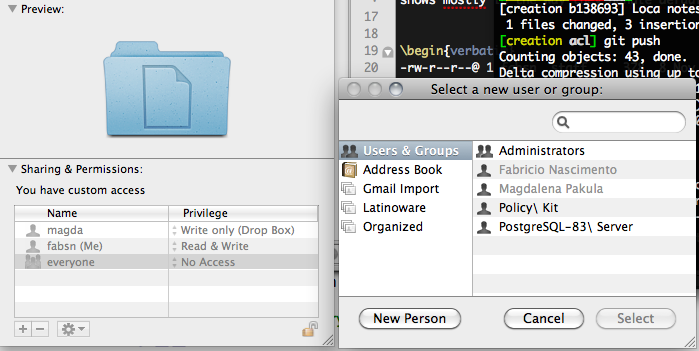
\includegraphics[height=3in]{img/mac-acl.png}
	\caption{Mac OSX Snow Leopard ACL Interface}
	\label{fig:img_mac-acl}
\end{figure}


%A voir maintenant

\subsection*{Using ACL in Linux}
 

The Linux getfacl and setfacl command line utilities do not strictly follow POSIX 1003.2c draft 17, which shows mostly in the way they handle default ACLs. See section 6.


\begin{verbatim}
-rw-r--r--@ 1 fabsn  staff     378  8 Nov 15:29 Makefile
-rw-r--r--@ 1 fabsn  staff     618  8 Nov 15:59 README
-rw-r--r--@ 1 fabsn  staff      31  8 Nov 15:15 draft-header
-rw-r--r--@ 1 fabsn  staff      24  8 Nov 15:15 header
drwxr-xr-x@ 2 fabsn  staff     102  8 Nov 15:26 img
-rw-r--r--  1 fabsn  staff     972  8 Nov 15:57 rapport-draft.aux
-rw-r--r--  1 fabsn  staff   18129  8 Nov 15:57 rapport-draft.log
\end{verbatim}

\begin{verbatim}
fabsn@vadmin:/media/esisar$ getfacl repertoire/
# file: repertoire/
# owner: root
# group: root
user::r-x
user:daemon:rwx
user:bin:rwx
user:fabsn:rwx
user:nobody:rwx
group::r-x
group:admin:rwx
group:fabsn:rwx
mask::rwx
other::r-x	
\end{verbatim}

%noyaux patches

% ls -l

%getfacl

%setfacl

%systemes de fichier
